% This is samplepaper.tex, a sample chapter demonstrating the
% LLNCS macro package for Springer Computer Science proceedings;
% Version 2.20 of 2017/10/04
%
\documentclass[runningheads]{llncs}
%
\usepackage{graphicx}
\usepackage{longtable}
\usepackage[usenames,dvipsnames]{xcolor}
\usepackage{wrapfig}

\newcommand*\ttvar[1]{\texttt{\expandafter\dottvar\detokenize{#1}\relax}}
\newcommand*\dottvar[1]{\ifx\relax#1\else
  \expandafter\ifx\string_#1\string_\allowbreak\else#1\fi
  \expandafter\dottvar\fi}
% Used for displaying a sample figure. If possible, figure files should
% be included in EPS format.
%
% If you use the hyperref package, please uncomment the following line
% to display URLs in blue roman font according to Springer's eBook style:
% \renewcommand\UrlFont{\color{blue}\rmfamily}

\begin{document}
%
\title{Towards automated provenance collection for experimental runs of agent-based models}

%\thanks{This work was supported by the Scottish Government Rural and Environment Science and Analytical Services Division (project reference JHI-C5-1)}}
%%% GP: if you ever want the standard acknowledgement text for C5, it's on our
%%% GP: project webpage at https://large-scale-modelling.hutton.ac.uk/
%
\titlerunning{An automated provenance collection framework}
% If the paper title is too long for the running head, you can set
% an abbreviated paper title here
%
\author{Doug Salt\inst{1} \orcidID{0000-0001-5186-9388} \and
 Gary Polhill\inst{1} \orcidID{0000-0002-8596-0590} \and
 Corran Musk\inst{1} \and
 Lorenzo Milazzo\inst{2} \and
 Dawn Parker\inst{3} \orcidID{0000-0001-8988-193X}  }

%%% GP: to discuss -- which other authors should we include here?
%%% GP: Kit Macleod? (Has he had intellectual input into this via WP1?)
%%% GP: Coran Musk? (Random acknowledgement for looking after the machines)
%%% GP: Lorenzo Milazzo? (As the original SSREPI developer)
%%% GP: Dawn Parker? (As MIRACLE PI -- do we see this as a MIRACLE paper?)
%
\authorrunning{D. Salt et al.}
% First names are abbreviated in the running head.
% If there are more than two authors, 'et al.' is used.
%
\institute{The James Hutton Institute, Craigiebuckler, Aberdeen, AB15 8QH, Scotland
\email{\{doug.salt,gary.polhill\}@hutton.ac.uk}\\
\url{https://www.hutton.ac.uk/}
\and Satellite and Surface Assimilation (SSA) Group
Met Office, FitzRoy Road, Exeter, Devon, EX1 3PB, UK
\email{lorenzo.milazzo@physics.org}
\and University of Waterloo, 200 University Avenue West
Waterloo, ON, Canada  N2L 3G1
\url{https://uwaterloo.ca/}
}
%
\maketitle              % typeset the header of the contribution
%
\begin{abstract}
    We demonstrate a working framework for the automatic recording of
    provenance and metadata for primarily agent-based models that could easily
    be adapted to the other modelling environments. We discuss the need for
    such a framework, the philosophy behind the design we adopted, the
    implementation, discuss the results and demonstrate a simple tool for for
    tracing bad data through a provenance graph.

\keywords{Provenance \and metadata \and modelling \and automation \and replication.}
\end{abstract}
%
%
%
\section{Introduction}

Replication of social simulation results has been highlighted as a significant
issue for the agent-based modelling (ABM) community for a number of years (e.g. \cite{edmonds2003replication}).
The paper that forms the basis of this work (\cite{polhill2017lessons}) shows that
the analysis of the outputs of the model can potentially be just as complex a
process as developing and running the model itself. Analysis of outputs is no less difficult
to replicate unless adequate records are kept. The TRACE protocol \cite{schmolke2010ecological,ayllon2021keeping} provides
some guidance highlighting the need to keep a notebook of the analysis done and
a standardised approach to making that notebook. There are also 
many scientific workflow tools, such as Snakemake
\cite{koster2012snakemake}, NextFlow \cite{di2017nextflow}, Kepler
\cite{ludascher2006scientific} and Taverna \cite{hull2006taverna}. However, since
these are workflow tools, the focus seems to be  on automation and
repeatability rather than provenance, which, if it is included, seems not to be the primary purpose of the described tools. There are exceptions to this, such as the open provenance framework \cite{moreau2008open}, implemented in \cite{gadelha2011provenance} with yet another workflow control langauge \cite{zhao2007swift}, but such tools do not seem to have flourished and seemingly for agent-based models are non existent.

One of the lessons learned from the replication exercise in
\cite{polhill2017lessons} was that, for the purposes of replication, more
detailed guidance on the information that should be recorded is needed. Since
recording such metadata is tedious (and error-prone) for humans, any such
guidance should be accompanied by specification of tools
that could be used to support the process. In the ideal world, the process
of recording provenance metadata would be completely automated, essentially providing a complete graph from data (including their sources) through applications (model, scripts and analysis tools, including versions thereof) to result.

The output analysis replication in this paper concerns earlier work with
FEARLUS-SPOMM, which is a coupled ABM of agricultural decision-
making and species stochastic patch occupancy metacommunity model that has been
used to explore incentivisation strategies to improve biodiversity
\cite{polhill_nonlinearities_2013,gimona2011exploring}. Belonging to the
‘typification’ class of social simulations  \cite{boero2005does}, this work
involved the analysis of the outputs of approximately 20,000 runs of the model
using a number of techniques aimed at demonstrating nonlinearities in the
relationship between incentivisation and biodiversity outcome.  Recording
provenance metadata on the process used to analyse and visualise the outputs is challenging, and
currently there are no codified standards as to how this should be done for
ABMs. For FEARLUS-SPOMM, the analysis and visualisation methods used drew heavily on statistical
techniques available as R packages.
Although R allows transcripts of interactive terminal sessions to be saved, the
work involved great deal of exploration of alternative analyses and visualisations, not all of
which were reported in the manuscript as finally accepted. Such transcripts are therefore not the
best way to record the means by which a model's outputs were analysed, and hence the
strategy used was to save each analysis or visualisation in a(n R) script.
Since the output from the (Swarm) model software used a mixture of text formats, some Perl scripts were also written to
process that output into CSV format for easy import into R. When the MIRACLE
project \cite{parker2019final} provided a context in which the replication of
that analysis was necessary, an opportunity was created to test the viability
of the strategy of relying on scripts to record provenance.

`Multifinality' (the same initial conditions and parameter settings having qualitatively different results) in ABMs means we need to ensure that
reported results are not just down to a matter of chance. This is one of many reasons (e.g. in empirical contexts especially, calibration, validation and sensitivity analysis) why experiments with ABMs involve large numbers of runs. The tedium (and in larger-scale cases, infeasibility) of conducting each run by hand means most ABM experiments resort to some kind of automation, including of the kind provided by workflow tools mentioned above, but also using built-in features of ABM software (e.g. in the case of NetLogo, BehaviorSpace). This is fine if all we
want to do is repeat the same process, but what if we are interested in why a particular instance of that process led to an unexpected outcome? Re-executing the workflow will not necessarily generate \textit{exactly} the same result unless we have a record of everything needed to do that (including seeds for pseudo-random number generators). We refer to this
as the `automation and replication' problem.  

%%% GP: Got here as at 2023-04-19T10:59.

%%% GP: Restarting 2023-05-11T15:36 -- these details on scripts can go and I am about to delete them

The automation of experiments is already solved by
\textit{scripting}. A script -- in a scripting language such as Python, Julia, or
Perl, but more typically an operating system `shell' language such as Bash --
records the sequence of programs that need to be executed to reproduce the experiment.
This at least repeats the
experiment, rather than \textit{precisely} replicating a specific set of results.
We believe that
anybody who does experiments with their agent-based models should at the
very least be scripting most of their experiments. In our experience the
preparation and the execution of the experiment is relatively straightforward
to script. Post-processing to the final data tables, diagrams, etc., that appear in
manuscripts and other documents should be included in these scripts. These scripts
can be conceived as \textit{workflow} metadata -- the means by which a \textit{class}
of outputs is achieved, rather than a specific instance.\footnote{In the case that all of the programs executed are deterministic, the class is a singleton.}

\textit{Provenance} metadata is used to record the means by which a specific output is achieved, which is more suitably stored in a 
database. That database is updated using a series of scripts written in Python, allowing us to develop on laptops and run
the resultant code in high-performance computing environments with little or
no reconfiguration. Bash scripts automating the experiment workflow are then modified to
call the Python scripts to update the provenance database. We implemented the database in Sqlite3 for local
development and PostgreSQL in high-performance infrastructure. In this way, we have created a provenance
tool that can record provenance during workflow execution.

\begin{figure} % wrapfigure is too small to see anything useful
    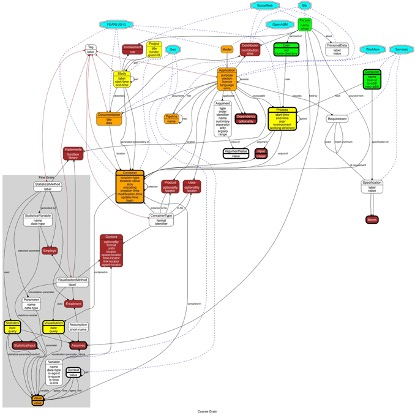
\includegraphics[width=\textwidth]{img/schema.jpeg} % You should use a PNG at >= 300 dpi; not a lossy format like JPEG. You can export PNGs from PDFs using Preview
\caption{SSREPI Schema} \label{fig:schema} \end{figure}

Another project adopting a similar approach is the \texttt{fair} data pipeline \cite{mitchell2022fair}, in which the provenance is automatically
recorded by embedded model code in R, C++, Java, Julia and Python. However, one of our requirements
was not to modify the model code if this could be avoided.\footnote{If the model code did not output the seed it used, then it would need to be modified.} In the example above, the FEARLUS-SPOMM model is written
in Objective-C \cite{objectivec}; with additional supporting Perl and R scripts to prepare the data and conduct the
post analysis. We would also prefer not to modify these scripts. Instead, we wrote wrapper scripts in Bash
\cite{bash4420}. A further observation is that our framework
generalises to more source metadata (papers, data, other experiments), and
is written with the requirements of agent-based modelling in mind first and foremost.

In the rest of this paper, we describe the scripting tool we have developed  for
automatically recording metadata, which can be incorporated into the analysis
replication process, and how this  was used to regenerate some of the figures
in \cite{polhill_nonlinearities_2013}. In addition we show a simple tool we have already developed to trace data through the provenance graph, and suggest additional work we would like to pursue.


\section{The \texttt{SSREPI} provenance and workflow tool}

One of the artefacts of the MIRACLE project \cite{parker2019final} was the
Social Simulation REplication Interface or \texttt{SSREPI}. This is the schema shown in
figure \ref{fig:schema}.  This schema has evolved since it original conception; 
\cite{polhill2022miracle} is the latest version. The schema is derived from the Dublin
Core \cite{weibel2000dublin} and PROV-O ontologies \cite{missier2013w3c} among others, and is designed with
agnosticism towards the underlying database technology, having been
implemented in PostgresSQL \cite{stonebraker1991postgres} and Sqlite3
\cite{sqliteorg2023syntax}.

Besides the distinction between workflow and provenance described above, we can discriminate
fine- versus coarse- grained metadata. Coarse-grained metadata describes how particular files come (or came) into
being, or were (or could be) used to bring other files into being. Fine-grained
metadata describes specific values recorded in social simulation outputs. To
make the distinction concrete, suppose a simulation produces a CSV file. The
data within the CSV file are covered by fine-grained metadata, whilst the fact
that the simulation produces the CSV file is coarse-grained. 

To build \texttt{SSREPI}, each table in schema shown in fig. \ref{fig:schema} was coded as an object type
in Python. Each table row was represented as an instance of such an object.
This design approach was adopted to enforce a consistent coding methodology
across all tables. To these were added a few simple coordinating commands that could be called from Bash:

\begin{itemize}
    \item {\color{OliveGreen} \ttvar{create_database.py}} - creates a
        database idempotently.
    \item {\color{OliveGreen} \ttvar{exists.py}} - checks
        if a particular row in a table exists.
    \item {\color{OliveGreen}
            \ttvar{get_value.py}} - gets any specified single value from a
            table given the primary key.
    \item {\color{OliveGreen} % 'green' hurt my eyes!
\ttvar{get_values.py}}  - gets one or more rows given the search values.
    \item {\color{OliveGreen}\ttvar{next_study.py}} - gets the next available and unique study number. \item
{\color{OliveGreen} \ttvar{update.py}} - idempotently updates a particular row in a
table.  \end{itemize}

`Idempotent' indicates that multiple operations on
the same entity will leave it unchanged after the initial operation. For
example multiplying something by 1 is idempotent. This allows for less
rigorous exception criteria, but implies that initialisation must be performed with care, as older data
will not necessarily be destroyed when overwritten with newer values, but
retain any values that already exist.\footnote{This is a design decision that may need revisiting.}

\begin{table}\begin{tabular}{|l|p{1cm}|p{5.5cm}|} \hline Primitive & Type & Purpose \\
    \hline {\color{blue} \ttvar{SSREPI_require_minimum}} & M & Lower
    bound on software hardware required \\ {\color{blue}
    \ttvar{SSREPI_require_exact}} & M & Exact bound on software
    hardware required \\ {\color{blue} \ttvar{SSREPI_application}} & P
    \& M & specifies some executable \\ {\color{blue} \ttvar{SSREPI_me}}
    & P \& M & Determines executable being run or returns a
    proper reference to the executable being run. \\ {\color{blue}
    \ttvar{SSREPI_argument}} & P & An argument type to an executable
    \\ {\color{blue} \ttvar{SSREPI_output}} & P & An output type from
    an executable \\ {\color{blue} \ttvar{SSREPI_input}} & P & An
    input type for an executable \\ {\color{blue}
    \ttvar{SSREPI_person}} & M & Provide metadata for a particular actor
    within this system\\ {\color{blue} \ttvar{SSREPI_project}} & M &
    Specifies a project which contains all studies \\ {\color{blue}
    \ttvar{SSREPI_study}} & M & A set of experiments makes up a single
    study \\ {\color{blue} \ttvar{SSREPI_set}} & M & Sets the default
    licence and other metadata \\ {\color{blue} \ttvar{SSREPI_involvement}} &
    M & Links personnel to a study \\ {\color{blue}
    \ttvar{SSREPI_paper}} & M & A paper associated with this study \\
    {\color{blue} \ttvar{SSREPI_make_tag}} & M & Used for building a
    folksonomy \\ {\color{blue} \ttvar{SSREPI_tag}} & M & Used to tag
    any entity with a folksonomy tag \\ {\color{blue}
    \ttvar{SSREPI_contributor}} & M & A  person with some kind of
    relation to an executable or script. \\

    {\color{blue} \ttvar{SSREPI_statistical_method}} & M & Record a statistical method \\ {\color{blue}
    \ttvar{SSREPI_visualisation}} & M & Record a method to create an image to depict one or more 
    values. \\
    {\color{blue} \ttvar{SSREPI_statistics}} & M & Record
    activities that compute and populate the values of statistical variables. \\ {\color{blue}
    \ttvar{SSREPI_visualisation_method}} & M & Methods
    for generating visualisations.
    \\
    
    {\color{blue} \ttvar{SSREPI_implements}} & M & Links a statistical
    or visualisation method to an application \\ {\color{blue}
    \ttvar{SSREPI_parameter}} & M & Record the name of a
    parameter taken by a statistical or visualisation method. \\ {\color{blue} \ttvar{SSREPI_statistical_variable}} &
    M &  A name for (one of) the result(s) of a statistical method. \\
    {\color{blue} \ttvar{SSREPI_visualisation_variable}} & P \&
    M & Declares a named variable of interest \\ {\color{blue}
    \ttvar{SSREPI_variable}} & M & Names a variable of interest \\
    {\color{blue} \ttvar{SSREPI_statistical_variable_value}} & P \&
    M & Sets an actual value for a named statistical variable \\
    {\color{blue} \ttvar{SSREPI_value}} & P & Sets a value.         \\ {\color{blue}
    \ttvar{SSREPI_content}} & M & Links a kind of output/input/argument
    to a variable  \\ {\color{blue} \ttvar{SSREPI_person_makes_assumption}} &
M & Links a person to an assumption \\ \hline \end{tabular} \caption{\texttt{SSREPI}'s Bash
commands for provenance (Type column entry `P') and other metadata (Type `M') recording} \label{tab:commands}
\end{table}

\normalsize

Each of the Bash commands listed in table \ref{tab:commands} composes over % What does 'composes over' mean?
the above Python commands to populate the \texttt{SSREPI} database in a consistent and
logical manner. Broadly speaking, {\color{blue} \ttvar{SSREPI_application}}, {\color{blue}
\ttvar{SSREPI_run}}, {\color{blue} \ttvar{SSREPI_batch}}, {\color{blue}
\ttvar{SSREPI_input}}, {\color{blue} \ttvar{SSREPI_output}} and {\color{blue}
\ttvar{SSREPI_argument}} are responsible for recording coarse grain provenance.
{\color{blue} \ttvar{SSREPI_value}}, {\color{blue}
\ttvar{SSREPI_visualisation_variable_value}}, {\color{blue}
\ttvar{SSREPI_statistical_variable_value}}, {\color{blue} \ttvar{SSREPI_run}}
and {\color{blue} \ttvar{SSREPI_batch}} record fine-grain provenance. The
remaining primitives are largely about recording other metadata. Further information may be found
in the tool's public repository. %\footnote{\url{https://github.com/DougSalt/ABM-metadata}}.

Using \texttt{SSREPI} for existing workflow scripts is a somewhat laborious task entailing adding calls to the provenance metadata scripts in Table \ref{tab:commands}. Improvements to the `interface' is the subject of future work.

\section{Demonstration}

Here, we demonstrate the use of \texttt{SSREPI} by repeating the experiment in
the paper \cite{polhill2017lessons}, showing some of the workflow and
provenance graphs, and then using fictitious examples to apply the workflow and
provenance metadata to addressing issues in large-scale experiments. From a
workflow perspective, the main result is that the principal diagrams in that
paper were successfully recreated, with the same, albeit not identical,
results. %right? % Plus, I've deleted all the whining :-)
% whoops the reviewer complained about there being nothing here, so I am going
% to have to reintrouduce some of the whining. :)
By this we mean that the diagrams produced for the original paper
\cite{polhill2017lessons} were "roughly the same". They were not identical, but
contained similar features close enough to illustrate the features that were originally reported on in the original research from
\cite{polhill2017lessons}.

After a run had completed successfully the database was run through several
supplementary programs to produce the following visualisations of the provenance metadata recorded:

\begin{itemize} \item \textbf{Analysis} - fine grain provenance pertaining to
            statistical and visualisation outputs.

        \item \textbf{Finegrain} - a provenance diagram down to the level of
        variables.  \item \textbf{Folksonomy} - a diagram showing annotations
            against the database, produced and categorised at the discretion of
            the user doing the annotation \item \textbf{Project} - management
            metadata. Largest granularity of metadata supported \item
            \textbf{Provenance} - provenance diagram at the level of file and
        parameter \item \textbf{Services} - service provided and requirement
            description \item \textbf{Workflow} - the actual workflow
\end{itemize}

The supplementary programs use the Dot language for input to Graphviz\cite{ellson2002graphviz}, producing the diagrams such as those in figures
\ref{fig:workflow}, \ref{fig:sub-provenance}, \ref{fig:broken-application} and
\ref{fig:high-lit-provenance-trace}. The workflow graph is in
fig. \ref{fig:workflow}. The resultant provenance graph is massive, since there were 20,000 runs (so 20,000 sets of outputs to record), so we only show a \textit{very small} section of the provenance graph in fig.
\ref{fig:sub-provenance}. 

\begin{figure} % I suggest you put 'dir = LR' in this DOT file -- we can't really read the workflow
\includegraphics[width=\textwidth]{img/workflow.pdf}
\caption{The workflow sub-graph} \label{fig:workflow} \end{figure}

\begin{figure}
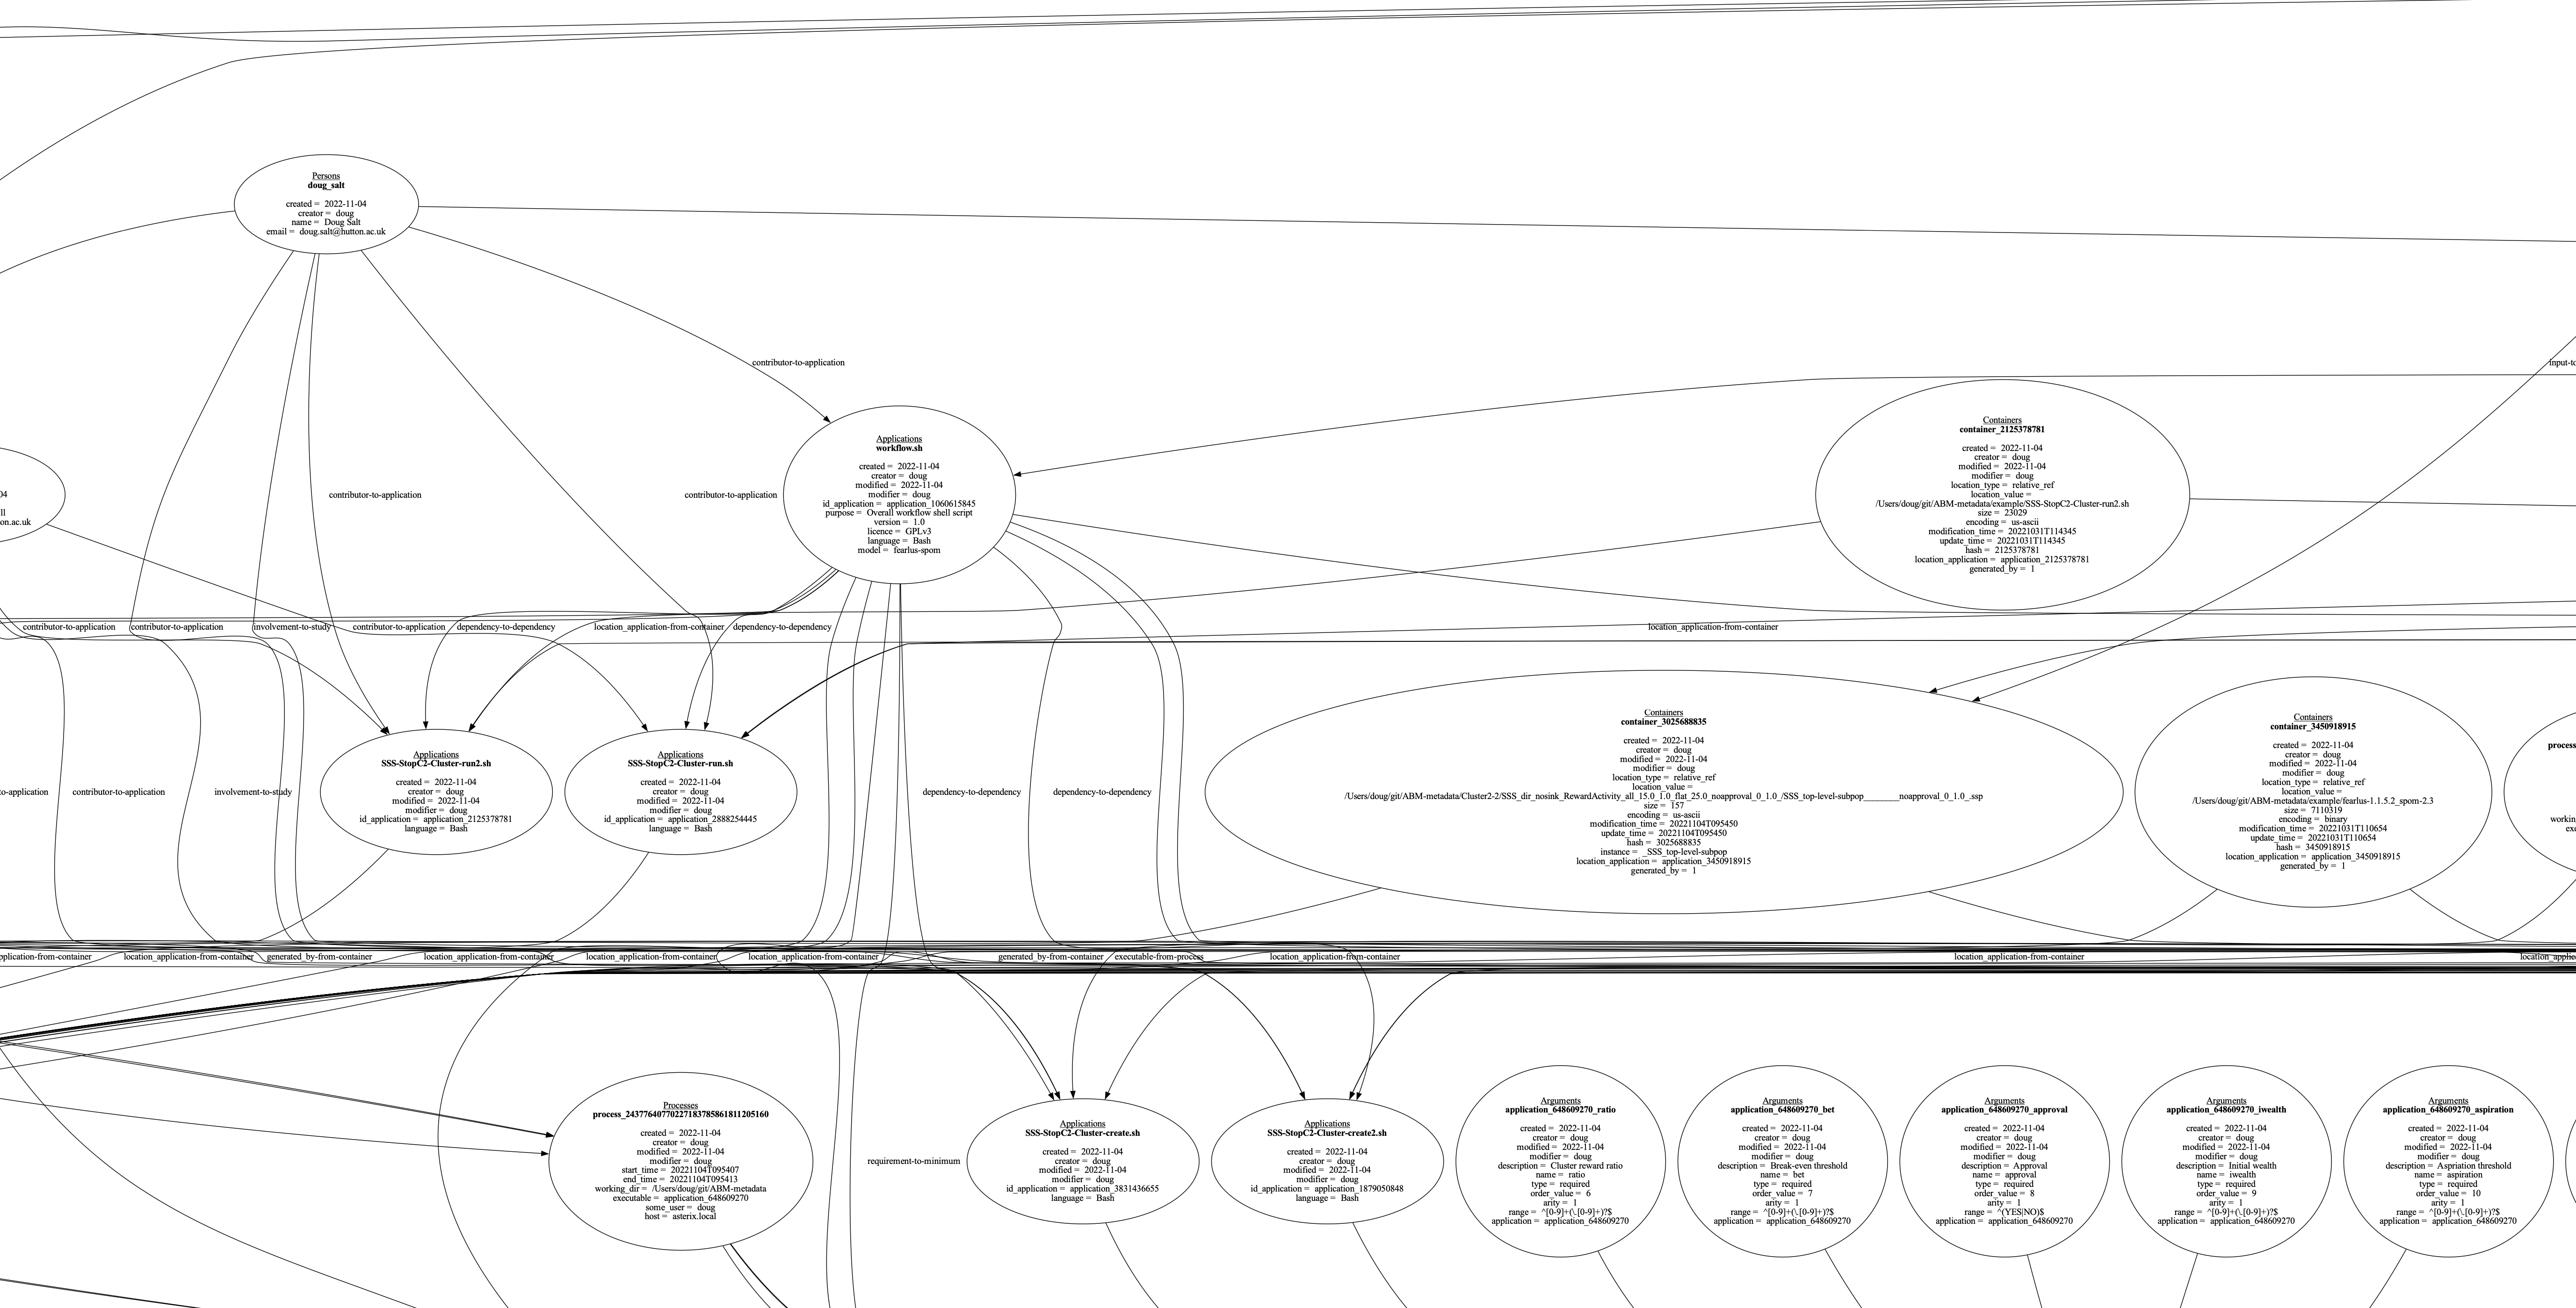
\includegraphics[width=\textwidth]{img/subsection-of-provenance.png}
\caption{A small sub-section of the provenance graph} \label{fig:sub-provenance}
\end{figure}

So what use is this provenance metadata? Imagine for the purposes of illustration that
we have found a bug in a script. The entity {\color{red}\ttvar{Applications.application_3831436655}} is an experiment setup script \ttvar{SSS-StopC2-Cluster-create.pl}. We can use the workflow graph to see what else in the workflow might be affected. As might be expected for an experiment setup script, there are serious cascading consequences, which we can visualise in Figure \ref{fig:broken-application}. The Dot language used by Graphviz constitutes a primitive graph
database. Indeed there are programs that can transform Dot files into TinkerPop
GraphSON format \cite{tinkerpop2015graphson,gv2graphson}, two reasonably well known and utilised graphing database formats. To generate Figure
\ref{fig:broken-application}, we used the workflow visualisation Dot file
rather than the relational database. 


\begin{figure} \includegraphics[width=\textwidth]{img/broken-application.pdf}
\caption{The workflow sub-graph show the propagation of a broken application (in red) to anything transitively making use of its outputs} \label{fig:broken-application} \end{figure}

Similarly, the provenance metadata can be used to check the damage caused to a large-scale experiment by a single bad dataset. In the real experiment, the input files are generated by running a script, but for the purposes of the example, suppose the data in
{\color{red}\ttvar{Containers.container_42949672955}} is wrong. The data in this file forms
a input file to a handful of runs, and we want an idea of how it has affected our results. We can visualise the propagation of the error in a \textit{very small} section of of the provenance graph in fig. \ref{fig:high-lit-provenance-trace}, but we can use the database to list the entities affected:

\tiny

\begin{table}
\begin{tabular}{ll}
	\ttvar{Applications.application_3450918915} &
	\ttvar{Applications.application_648609270} \\
	\ttvar{Computers.asterix.local} &
	\ttvar{Containers.container_1814970370} \\
	\ttvar{Containers.container_1982026419} &
	\ttvar{Containers.container_2050039078} \\
	\ttvar{Containers.container_2056384913} &
	\ttvar{Containers.container_2060874102} \\
	\ttvar{Containers.container_2387213333} &
	\ttvar{Containers.container_2486610989} \\
	\ttvar{Containers.container_2582525701} &
	\ttvar{Containers.container_2759060318} \\
	\ttvar{Containers.container_2865400753} &
	\ttvar{Containers.container_3025688835} \\
	\ttvar{Containers.container_3307537171} &
	\ttvar{Containers.container_3470971297} \\
	\ttvar{Containers.container_354343442} &
	\ttvar{Containers.container_4235735972} \\
	\ttvar{Containers.container_4294967295} &
	\ttvar{Containers.container_441913555} \\
	\ttvar{Containers.container_505627104} &
	\ttvar{Containers.container_800277554} \\
	\ttvar{Containers.container_878886043} &
	\ttvar{Containers.container_900718909} \\
	\ttvar{Persons.doug} &
	\ttvar{Persons.doug_salt} \\
	\ttvar{Processes.process_232221298886493}... &
	\ttvar{Processes.process_326475499597022}... \\
	\ttvar{Specifications.R} &
	\ttvar{Specifications.bash} \\
	\ttvar{Specifications.cpus} &
	\ttvar{Specifications.disk_space} \\
	\ttvar{Specifications.memory} &
	\ttvar{Specifications.os} \\
	\ttvar{Specifications.perl} &
	\ttvar{Specifications.python} \\
	\ttvar{Studies.1} &
	\ttvar{Users.doug}
 \end{tabular}
\end{table}

\normalsize

Having done so, we are then in a position to fix the data file, and rerun only that part of the workflow needed to regenerate the affected containers.

\begin{figure} \includegraphics[width=\textwidth]{img/high-lit-provenance-trace.pdf}
\caption{A provenance sub-graph showing (in red) the propagation of bad data through the system} \label{fig:high-lit-provenance-trace} \end{figure}

\section{Discussion}

It might seem that we are confusing random stream control and reproducibility
of individual simulation runs, i.e., given a set of inputs and random stream
that the simulation would always produce the same results, versus the
reproducibility of an overall analysis that comes out of a calibration or other
simulation workflow. However, the latter issues cannot even begin to be
addressed until a reproducible and reliable workflow is implmented for agent based models -
that is a directed acyclic graph from inputs to published outputs/visualisation
and/or results. This may seem like a contradiction to our earlier claim that
this is not a workflow tool, but workflow in agent-based models is complex and
the link from data/model to published material for agent-based models is
currently missing. Agent based modelling does not have any specialist needs in
terms of work control other than magnitude on the number of inputs, number of
runs and number of resuts. However step ups in magnitude are not always trivial
as the step up petaflop to exaflop is demonstrates
\cite{north2008agent}.



\section{Future work}

Provenance should be a directed acyclic graph. As the schema stands, it does not
guarantee that the graph is acyclic. In future work, we can  normalise the
schema to remove redundancy and the conflicts arising therefrom;
and once this complete, we can formally prove the schema to be acyclic. 
Until the schema is formally analysed, then we can not say with confidence that
any recorded provenance is not inherently contradictory. Since such a schema is likely to be
iteratively revised if the underlying provenance model changes or additional
functionality is required, then it would be advisable to automate such proving
of consistency (assuming correct normalisation). 

We should probably be using a graphing language such as Gremlin \cite{rodriguez2015gremlin}. The
advantages of using graphing databases over relational databases is that such
languages are inherently designed to store, traverse and query the graphs that
are the main product of this framework. This makes querying in such languages
trivial and fast. In a relational databases the SQL statement to do this are
cumbersome, awkward and probably (human) error-prone given their size and complexity to construct. Moreover on huge
datasets they are reportedly slow. Relational databases do have the advantage
of being an extremely mature technology and the availability of utilities that
implies. A further advantage of using relational databases is that
Structured Query Language is standard for all such databases, and therefore
queries written for any relational database should be the same. A tool we
already use, Graphviz, already does act like a graphing database language to a
certain extent. Indeed we used the Graphviz Dot files produced by the visualisation supplementary programs, rather than the
relational schema, in our simple examples to trace bad data through our
provenance graphs.  However the Dot language of Graphviz is primarily
purposed as a diagramming language and lacks the sophistication, such as a
built-in query language of say, Gremlin.

We would eventually like to take many provenance databases run some machine learning across them to see if there are any commonalities. We hope to uncover similarities in setup, execution and post-processing that could form core, reusable and proven components for primarily agent-based modelling but also for other modelling frameworks. These can then be used to \textit{suggest} workflow -- e.g. given files of these kinds, what have others done to visualise them?

The plan is to adapt this provenance framework to other model running language
frameworks, in particular R, Python, Julia, Java and thence NetLogo. This would
take the approach of the \texttt{fair} data pipeline \cite{mitchell2022fair}, but unlike
the example we have presented here such provenance would be embedded in the
experiments as a matter of course. In the meantime, our demonstration with FEARLUS-SPOMM shows that the \texttt{SSREPI} provenance framework may be `retrofitted' to existing
experiments (although possibly at the cost of the programmer's sanity with the present interface), and we can successfully repeat the published experiment. In the short-term, we have tentative potential adopters using R and Python as their primary modelling language.

% ---- Bibliography ----
%
% BibTeX users should specify bibliography style 'splncs04'.
% References will then be sorted and formatted in the correct style.
%
\bibliographystyle{splncs04}
\bibliography{global.bib}
% \bibliography[keyword={github.com/DougSalt/SSC2023}]{global.bib}
%
\end{document}
